\chapter{Act I}



\begin{figure}
    \centering
    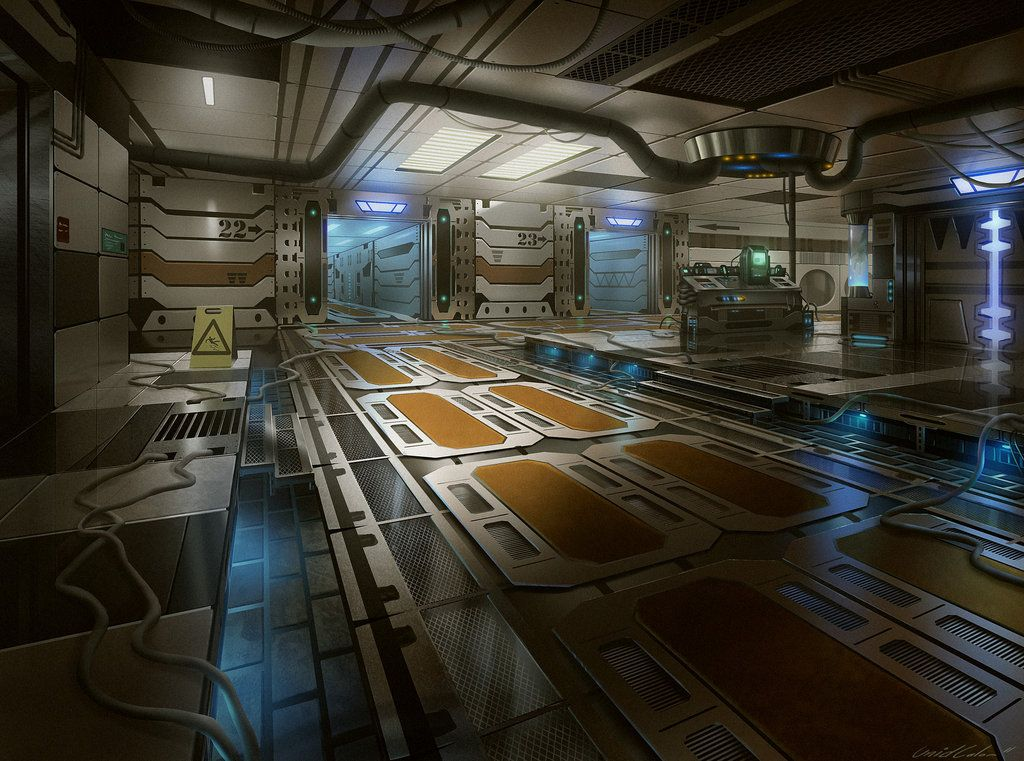
\includegraphics[width=.45\textwidth]{img/bg/interior.jpg}
\end{figure}



\begin{rpg-commentbox}{}

    Corporate people arrive at the station and \pc{Kathia} wants to bring a \pc{PC} back to Lasalle Bionational territory. She speaks with the station marshal Abdul Mageed and is allowed to take the elevator down to refinery levels where she can talk with the prisoner.

    Either all or part of her crew go down with her to ensure her security (Mik and Victor) or to play some role in the extraction (Tery and Aleki). 
    
\end{rpg-commentbox}


% \medskip
% \begin{rpg-commentbox}{Lasalle Objectives}
% If you plan to run the adventure using the crew make sure that either no one follows Kathia to prison OR that players are equally divided between station and prison levels.

% \begin{itemize}
%     \item Potential introductions

%     \item Negotiation between the Lasalle and Kohru crews. \textbf{manipulation} \textbf{command}
% \end{itemize}
% \end{rpg-commentbox}



\medskip
\begin{rpg-commentbox}{Prisoner Objectives}
For the prisoners, keep them busy dividing them either at the mining area or the refinery area. Some events to serve as ice breakers:

\begin{itemize}
    \item There is a solar glass panel that is not protecting against ultraviolet radiation in the refinery. Part of the crew should fix that. An entire shift can fix a small portion of the panel but not everything. This will have a role later on. \textbf{heavy machinery}

    \item Rumors spread that there is a synthetic amongst the prisoners and people plot how to rule out who is the synthetic to feed misinformation to it \textbf{observation}

    \item A potential murder attempt among the prisoners \textbf{close combat}

    \item Bartering among prisoners \textbf{manipulation}
\end{itemize}
\end{rpg-commentbox}


\newsect

\section{Station Lockdown}



\begin{rpg-commentbox}{}
    
    Within some of the lithium ore, there are parasite spores created by the engineers. When the ore is heat and pulverized in the refinery section, a small parcel of the parasites spread through the station ducts. Two will make their way to hosts in the refinery section while a third one will infect someone at the crew quarters. 
    
    The Kohru computer system, \textbf{Dexter}, warns about environmental hazard contamination and puts the station in lockdown. Increase stress level by 1
\end{rpg-commentbox}    


\medskip
\begin{rpg-commentbox}{Notes for potential escape plans}
\begin{itemize}
    \item The only person with a corporate key card is at the prison (Kathia). The card is necessary to turn the engines of the Lasalle Bionational ship back online if anyone plans to escape. The keycard is \textbf{either} in Kathia's possession or locked under some biometric safe with instructions to corrupt the card if anyone tries to crack it open. 

    \item It's also necessary to open the landing hatch. Potential solutions involve using the sulfuric acid in the refinery or blowing the thing open. Either option will take the air out of the refinery and if done before the keycard is retrieved, that will put all future events on a timer. I advise to run for air supply periodically.
\end{itemize}
\end{rpg-commentbox}


% \begin{quotation}
% \begin{small}
% \textit{}

% \textit{}    
% \end{small}    
% \end{quotation}
    


\newsect

\newpage

\section{Escape plan}


\begin{rpg-commentbox}{}
    Lock-down won't let the elevator between the levels work until environment measurements are back to standard levels.
    
    
    The prisoners can check air filters at several locations to make sure the station's system is not just malfunctioning. In fact this is not the first time that something similar has happened. At some point, one of the prisioners will be brought back to medical where he start having convulsions...

\end{rpg-commentbox}

\begin{rpg-commentbox}{The Alien}
    This is also a good place for foreshadowing. Describe via radio communication some prisoners saying that some strange ore was found in the pulverizer or things that allude to an extra presence in the prison ward.
 \end{rpg-commentbox}




\begin{rpg-commentbox}{Infection stages}
    \begin{enumerate}
        \item convulsions and med bay
        \item splitting blood and more seizures
        \item host's death
    \end{enumerate}

    At this point, players are probably expecting the creature to burst out of the host. However, it won't happen and the spore will keep growing and merging its DNA with the hosts. Let them discuss and imagine whether this was a heart attack or something else. All initial attempts will point to a normal disease and equipment for an autopsy is only available at the upper level.  \textbf{medical aid}

\end{rpg-commentbox}





\newsect

\section{Heated discussion}


\begin{rpg-commentbox}{}
    
    Draw the players' attention somewhere else other than the dead body. If one player decides to stay behind and watch for the corpse, this may have several consequences in the game and a potential early death.
    
    -- A potential event is a discussion in the intercon between Kathia and Mageed, where Kathia desperately tries to convince him of escorting her out of the prison ward \textbf{manipulation}
    
    -- Tery can also reveal his hidden camera and say that he has footage that could ruin the Marshal's career

\end{rpg-commentbox}

\newsect



\begin{rpg-commentbox}{Fresh meat in the prison block}
    
    Negotiation to escape the prison ward is not successful. When players get back to the dead body's location, it is missing. Increase stress level by 1.
    
    There is a trail of blood leading into either the refinery direction or the mines. If one of the players stayed behind they witness:
    
    \textit{
    ``The alien is parasitic. It is still feeding from the host and using its motor system while it grows stronger. At this stage, players can see a protuberance in the person's back, exposed insect like tendrils ripping through the flesh, broken bones, and four long and thin spider-like appendages sprouting from the the host's back. The creature uses these sharp appendages to attack and kill potential threats or to infect new victims''.
    } 

    \medskip
    
    
    Roll a combat scene between any players that stayed behind and the creature. \textbf{Alien is at stage I (host attached)}
    
    If attacked and threatened, the creature can detach from the host and escape thorough an air duct. It will eventually find a new host in the mines.
    
    

\end{rpg-commentbox}    


\begin{rpg-commentbox}{Corporate security comes first}
    Kathia will persuade the prisoners to safeguard her and take her out of the station. Any prisoners protecting her will receive new identities in Lasalle Bionational controlled space.
\end{rpg-commentbox}
    


\begin{rpg-commentbox}{End of Act}
    \textbf{Act 1 ends when prisoners notice the missing body OR fight the stage I alien.}
 \end{rpg-commentbox}